\documentclass[11pt,a4paper]{article}
\usepackage{fullpage}
\usepackage{amsmath}
\usepackage{amssymb}
\usepackage{amsfonts}
\usepackage{mathtools}
\usepackage{titlesec}
\usepackage{graphicx}
\usepackage{float}
\usepackage{wrapfig}
\usepackage{multicol}
\usepackage{caption}
\usepackage{hyperref}
\usepackage{apacite}
\usepackage{multirow}

\titleformat*{\section}{\large\bfseries}

\begin{document}
	
	\title{\textbf{Master Project \\ Computer Graphics: Rendering Track}}
	\author{\textbf{Alhajras Algdairy} \\ \textbf{Advisor: Prof. 
			Dr.-Ing. Matthias Teschner}}
	\maketitle
	
	\section*{\centering Acknowledgment}
	I want to express my special thanks of gratitude to Prof. Dr.-Ing. Matthias Teschner, who guided me through my master's program in general and in this master's project in specific. This project gave me the golden opportunity to dig into an exciting topic in computer graphics that I am keen on. The flexibility in research made me learn more about the related topics I am interested in, in rendering. Reading scientific topics and reviewing codes from different repositories expanded my expertise, where I had a full responsibility to control my time and resources, to learn more about the research process. 	
	
	\section*{\centering Abstract}
	This report investigates four different acceleration data-structure methods for implementing a simple raytracer on CPU. These methods are KD-tree, Uniformgrid, BVH, and LBVH. The report aims to compare the different approaches and their impact on the raytracer rendering time. The raytracer used in this project builds upon a previous lab project where the foundation of the raytracer is already implemented; however, without using a sophisticated data-structure to enhance the rending performance; hence the focus of this report will be how to improve the raytracer performance by using data-structures. 
	\textbf{\textit{Keywords: Ray Tracing; kD-Tree; BVH; LBVH; Uniformgird; Data structure;}}
	
	\section{Introduction}
	This report summarises my journey to implement a simple raytracer focusing on data structure level, where the performance of rending a scene will be the lion's share of the report. Theory, implementation, and results will be discussed in depth in the report, where an introduction and motivation of what is raytracer and how to implement it will be briefly discussed; because data structures are more interesting for us, I will only explain the topics that are used in this raytracer. 
	
	\section{What is Raytrcer and how it works}
	
	
	
	In Computer Graphics, scientists are interested in simulating a real-life phenomenon, such as Gravity Fraction, Rain, Snow, and the exciting part for us, light.  Simulating light is arguably the most challenging part because light has always been difficult to characterize as it can behave as particles and waves, which makes it spread into the whole scene based on probabilities. This makes it difficult to compute as it involves complex computation and infinite simulations to execute to have a perfect result without an error.
	
	Why do we need to simulate light? Adding light into a scene will generate shadows, reflection, and refraction consequently will illuminate the scene, making the scene look like a reality, which can be helpful for some applications. For the internal designers, it is vital to simulate the final result of the lightning inside a room, such as sunlight coming from the windows, the light of lamps, and fireplace, these with react together and create shadows, before constructing the building and payloads of money, simulating the right angle and place of the room is helpful to imagine the final result. Solar engineers use 3D tools to build solar panel farms where the angle between the sunlight and the panel is essential to gather as much light energy as possible. In gaming, different companies compete to design engines that can produce natural scenes; this includes lighting and shadowing.  
	
		\begin{figure}[H]
		\begin{center}
		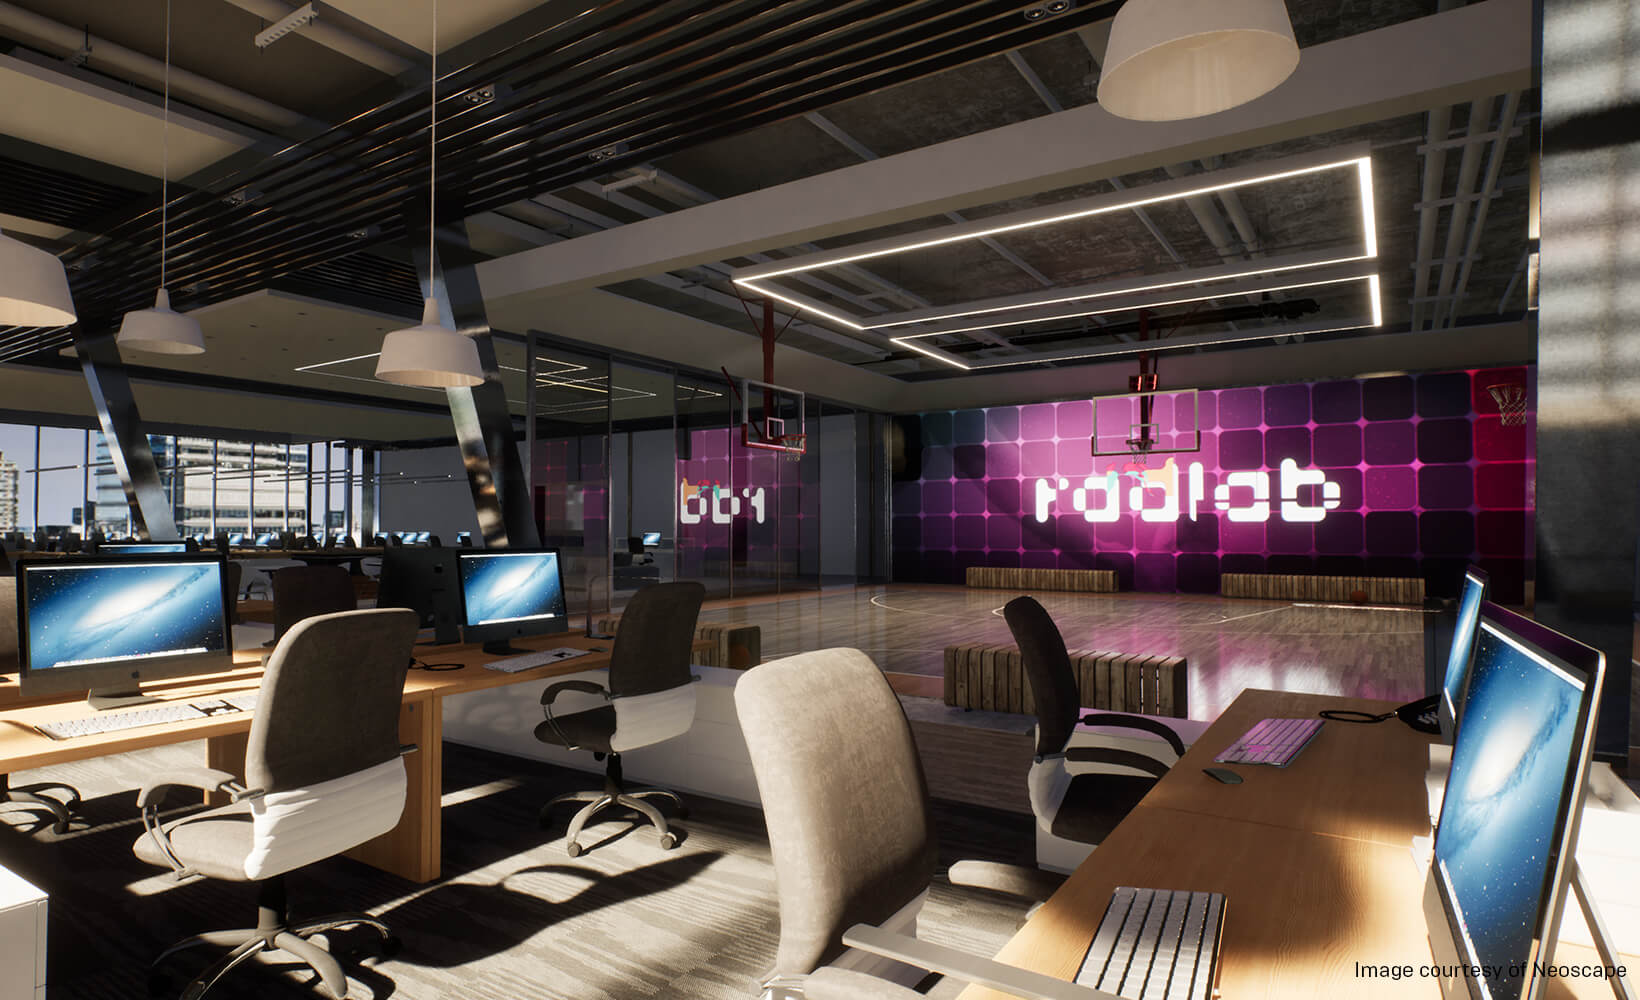
\includegraphics[width=0.7\textwidth]{2.jpg}
			
			\caption{https://www.pcgamer.com/unreal-engine-5-tech-demo-pc-performance/ The raytracing algorithm builds an image by extending rays into a scene and bouncing them off surfaces and towards sources of light to approximate the color value of pixels [Piotr Dubla, "Interactive Global Illumination on the CPU."
				]}
			\label{fig:1}
		\end{center}
	\end{figure}
	
		\begin{figure}[H]
		\begin{center}
					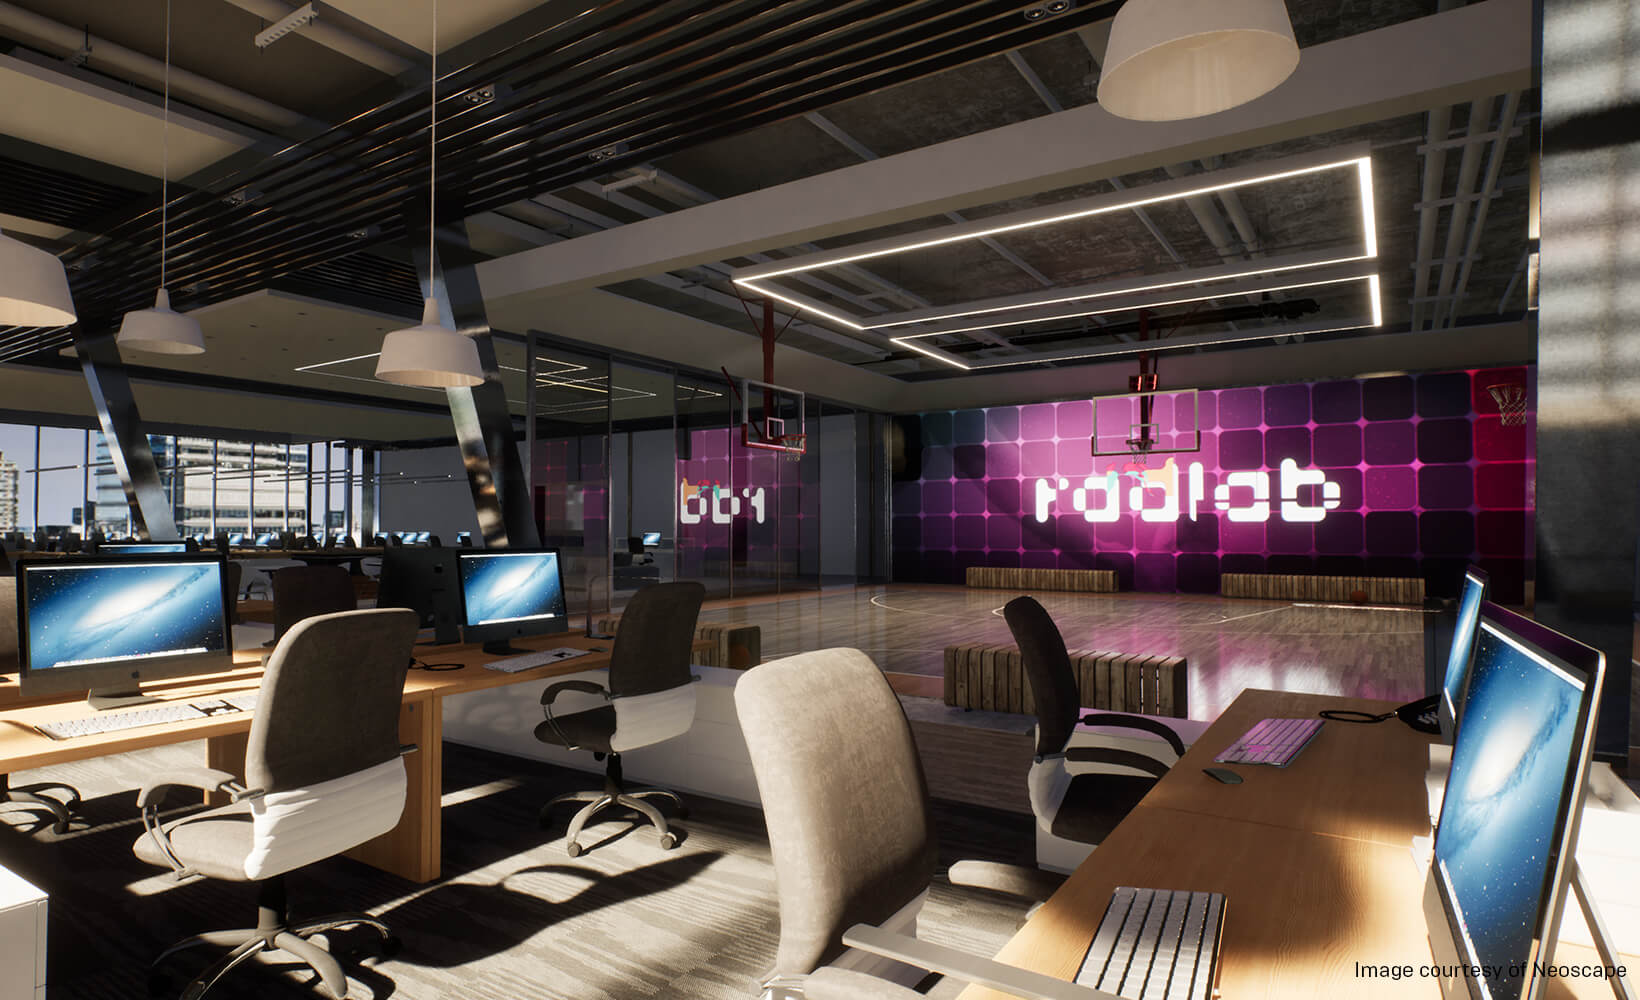
\includegraphics[width=0.7\textwidth]{2.jpg}
			
			\caption{ https://www.unrealengine.com/en-US/blog/real-time-ray-tracing-in-unreal-engine---part-2-architectural-visualization [Piotr Dubla, "Interactive Global Illumination on the CPU."
				]}
			\label{fig:1}
		\end{center}
	\end{figure}

		\begin{figure}[H]
	\begin{center}
		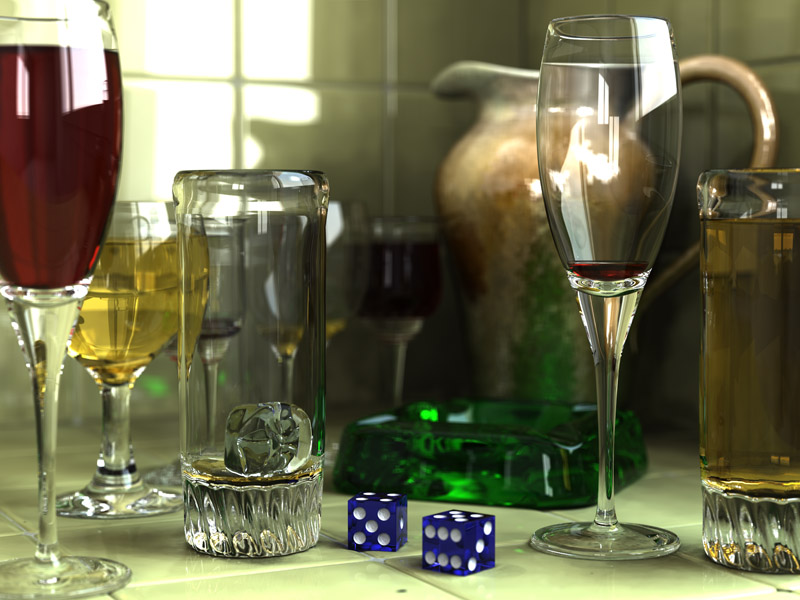
\includegraphics[width=0.7\textwidth]{1.jpg}
		
		\caption{ $ http://www.oyonale.com/modeles.php$ }
		\label{fig:1}
	\end{center}
\end{figure}
	
	
	
	
	
	Raytracing is a rendering technique that may provide extremely lifelike lighting effects. In other words, an algorithm can track the source of light and then mimic how the light interacts with the virtual objects it eventually encounters in the computer-generated environment. Raytracing produces far more lifelike shadows and reflections, as well as significantly enhanced translucence and dispersion. The algorithm considers where the light falls and calculates the interaction and interplay in the same way as the human eye does with actual light, shadows, and reflections. The way light interacts with items in the world has an impact on the colors you perceive.
	
	\vspace*{5px}
	Raytracer involves in different industries and applications. The media uses it because Raytracing can be beneficial in theater and television lighting since it allows for visually accurate simulation of light. Engineers also use the technique to forecast light levels, brightness gradients, and visual performance requirements in the following fields: Simulations, Modelling tools, and architectures. 
	
	\vspace*{5px}
	To render a scene by the Raytracer, three crucial steps must be followed: 
	\textit{Casting Rays}: cast a ray for each pixel in the image.
	\textit{Path tracing}: check if a ray crosses any of the scene's objects using the ray-geometry intersection, and trace the ray back to the source.
	\textit{Shading}: determine how the object looks (color and brightness) at the point where the ray intersects the object.
	
	\vspace*{5px}
	Raytracing has two main methods: 
	\begin{itemize}
		\item 		\textit{Forward Raytracing}: The light particles (photons) are tracked from the light source to the object via Forward Raytracing. While forward ray tracing is the most exact method for determining the color of each object, it is also the most inefficient.
		\item 		\textit{Backward Raytracing}: 
		An eye ray is formed at the eye in backward ray tracing, and it travels through the viewplane and out into the scene. If it hits an object, it will return it to the viewplane immediately. This method is more efficient than Forward Raytracing but less accurate due to reducing the rays used. In this implementation this method is used.
	\end{itemize}
	
	Computer graphics has three main pillars: \textit{Modelling}, \textit{Rendering}, and \textit{Simulation}. The focus of this report is Rendering. Rendering cares about solving issues like the model's visibility towards sensors; this is done by two methods: \textit{Rasterization} or \textit{Raytracing}, this report is about a Raytracer implementation. Rendering also focuses on which color and intensity does a model has. How light interacts with surfaces and how it propagates throw the media.
	\section{Object subdivision}
	\section{Spatial Subdivision}
	
	This lab was a great way to gain practical experience of the concepts we learned in our computer graphics course. I would like to thank \textbf{Prof. Dr.-Ing. Matthias Teschner} again for advising me throughout this lab. As a final remark, I would like to mention that I really enjoyed working on area lights. This includes debugging issues as I was working on them as well as how they were fixed. At the end, the results were worth the effort.
	
	\bibliographystyle{apacite}
	\bibliography{References}
	
\end{document}